\chapter{Testing \label{chap:testing}}

\label{chap:testing}

\epigraph{All life is an experiment. The more experiments you make the better.}{\textit{Ralph Waldo Emerson \\ American essayist }}

Firstly, this chapter deals with the simulation of the LSP process in RoboDK. Secondly, it focuses on testing the robotic arm program on the physical robotic arm. The goal of the testing is to evaluate the effectiveness of the solution realised in the CAM program RoboDK. The robotic arm cell used for simulation and testing is depicted in \hyperref[sec:lsp_layout]{section \ref{sec:lsp_layout} -- LSP station layout}. A~forging die is used as a~test sample. Figure~\ref{fig:cad} shows a~CAD drawing of the forging die. Figure~\ref{fig:cad} also highlights the areas to be treated by the LSP process in black and the approach/retreat motions in green. The area treated by LSP is made up of a~line of consecutive laser shots. Information about the location of the areas to be treated by the LSP process is usually provided by the manufacturers based on experience from the factory floor. The actual testing described in this chapter was done with the Litron LPY~ST~7875-10~2HG laser and the FANUC~M-20iA/20M robotic arm. 



\section{Simulation}

The simulation process can be broken down into several steps:

\begin{enumerate}

\item create a~robot machining project in RoboDK, so it mirrors the actual robotic arm workcell, 

\item set up the curve follow project, set appropriate collision checking parameters and successfully solve robotic arm path,

\item set appropriate simulation parameters and run simulation,
generate robotic arm program with RoboDK,

\item if simulation is successful, continue with testing on physical robotic arm.

\end{enumerate}

\begin{figure}[h]
    \centering
    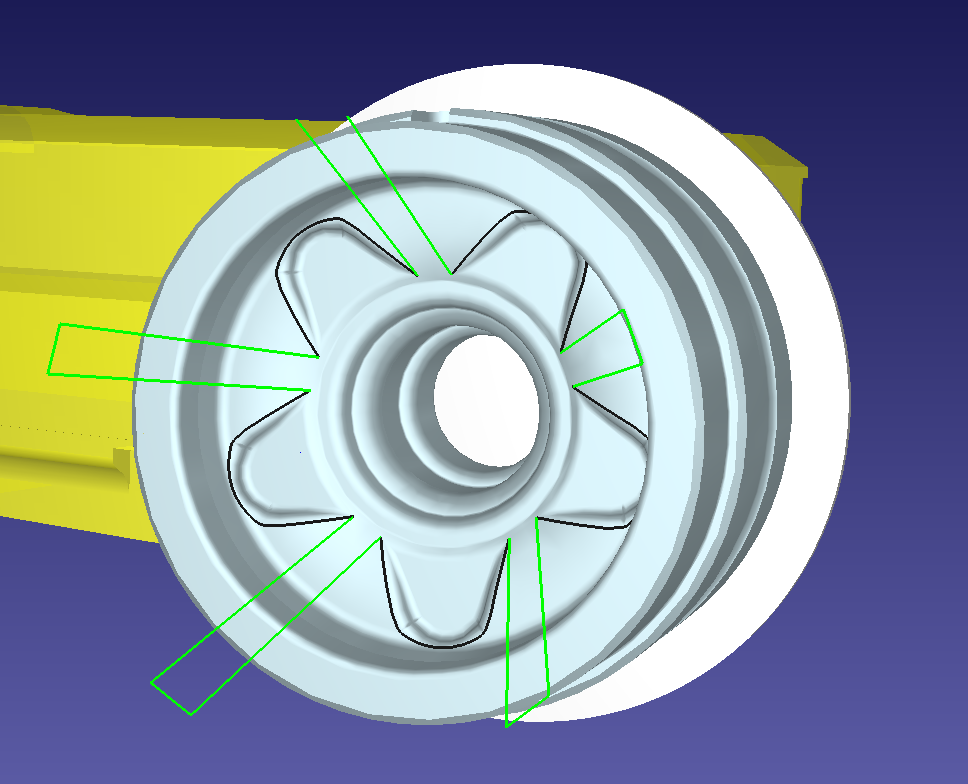
\includegraphics[width=0.5\linewidth]{img/cad.PNG}
    \caption{CAD drawing of forging die}
    \label{fig:cad}
\end{figure}
\noindent Figure~\ref{fig:robodk_die} shows a~picture of the RoboDK workcell with the forging die mounted onto the flange of the FANUC~M-20iA/20M robotic arm.

\begin{figure}[h!]
    \centering
    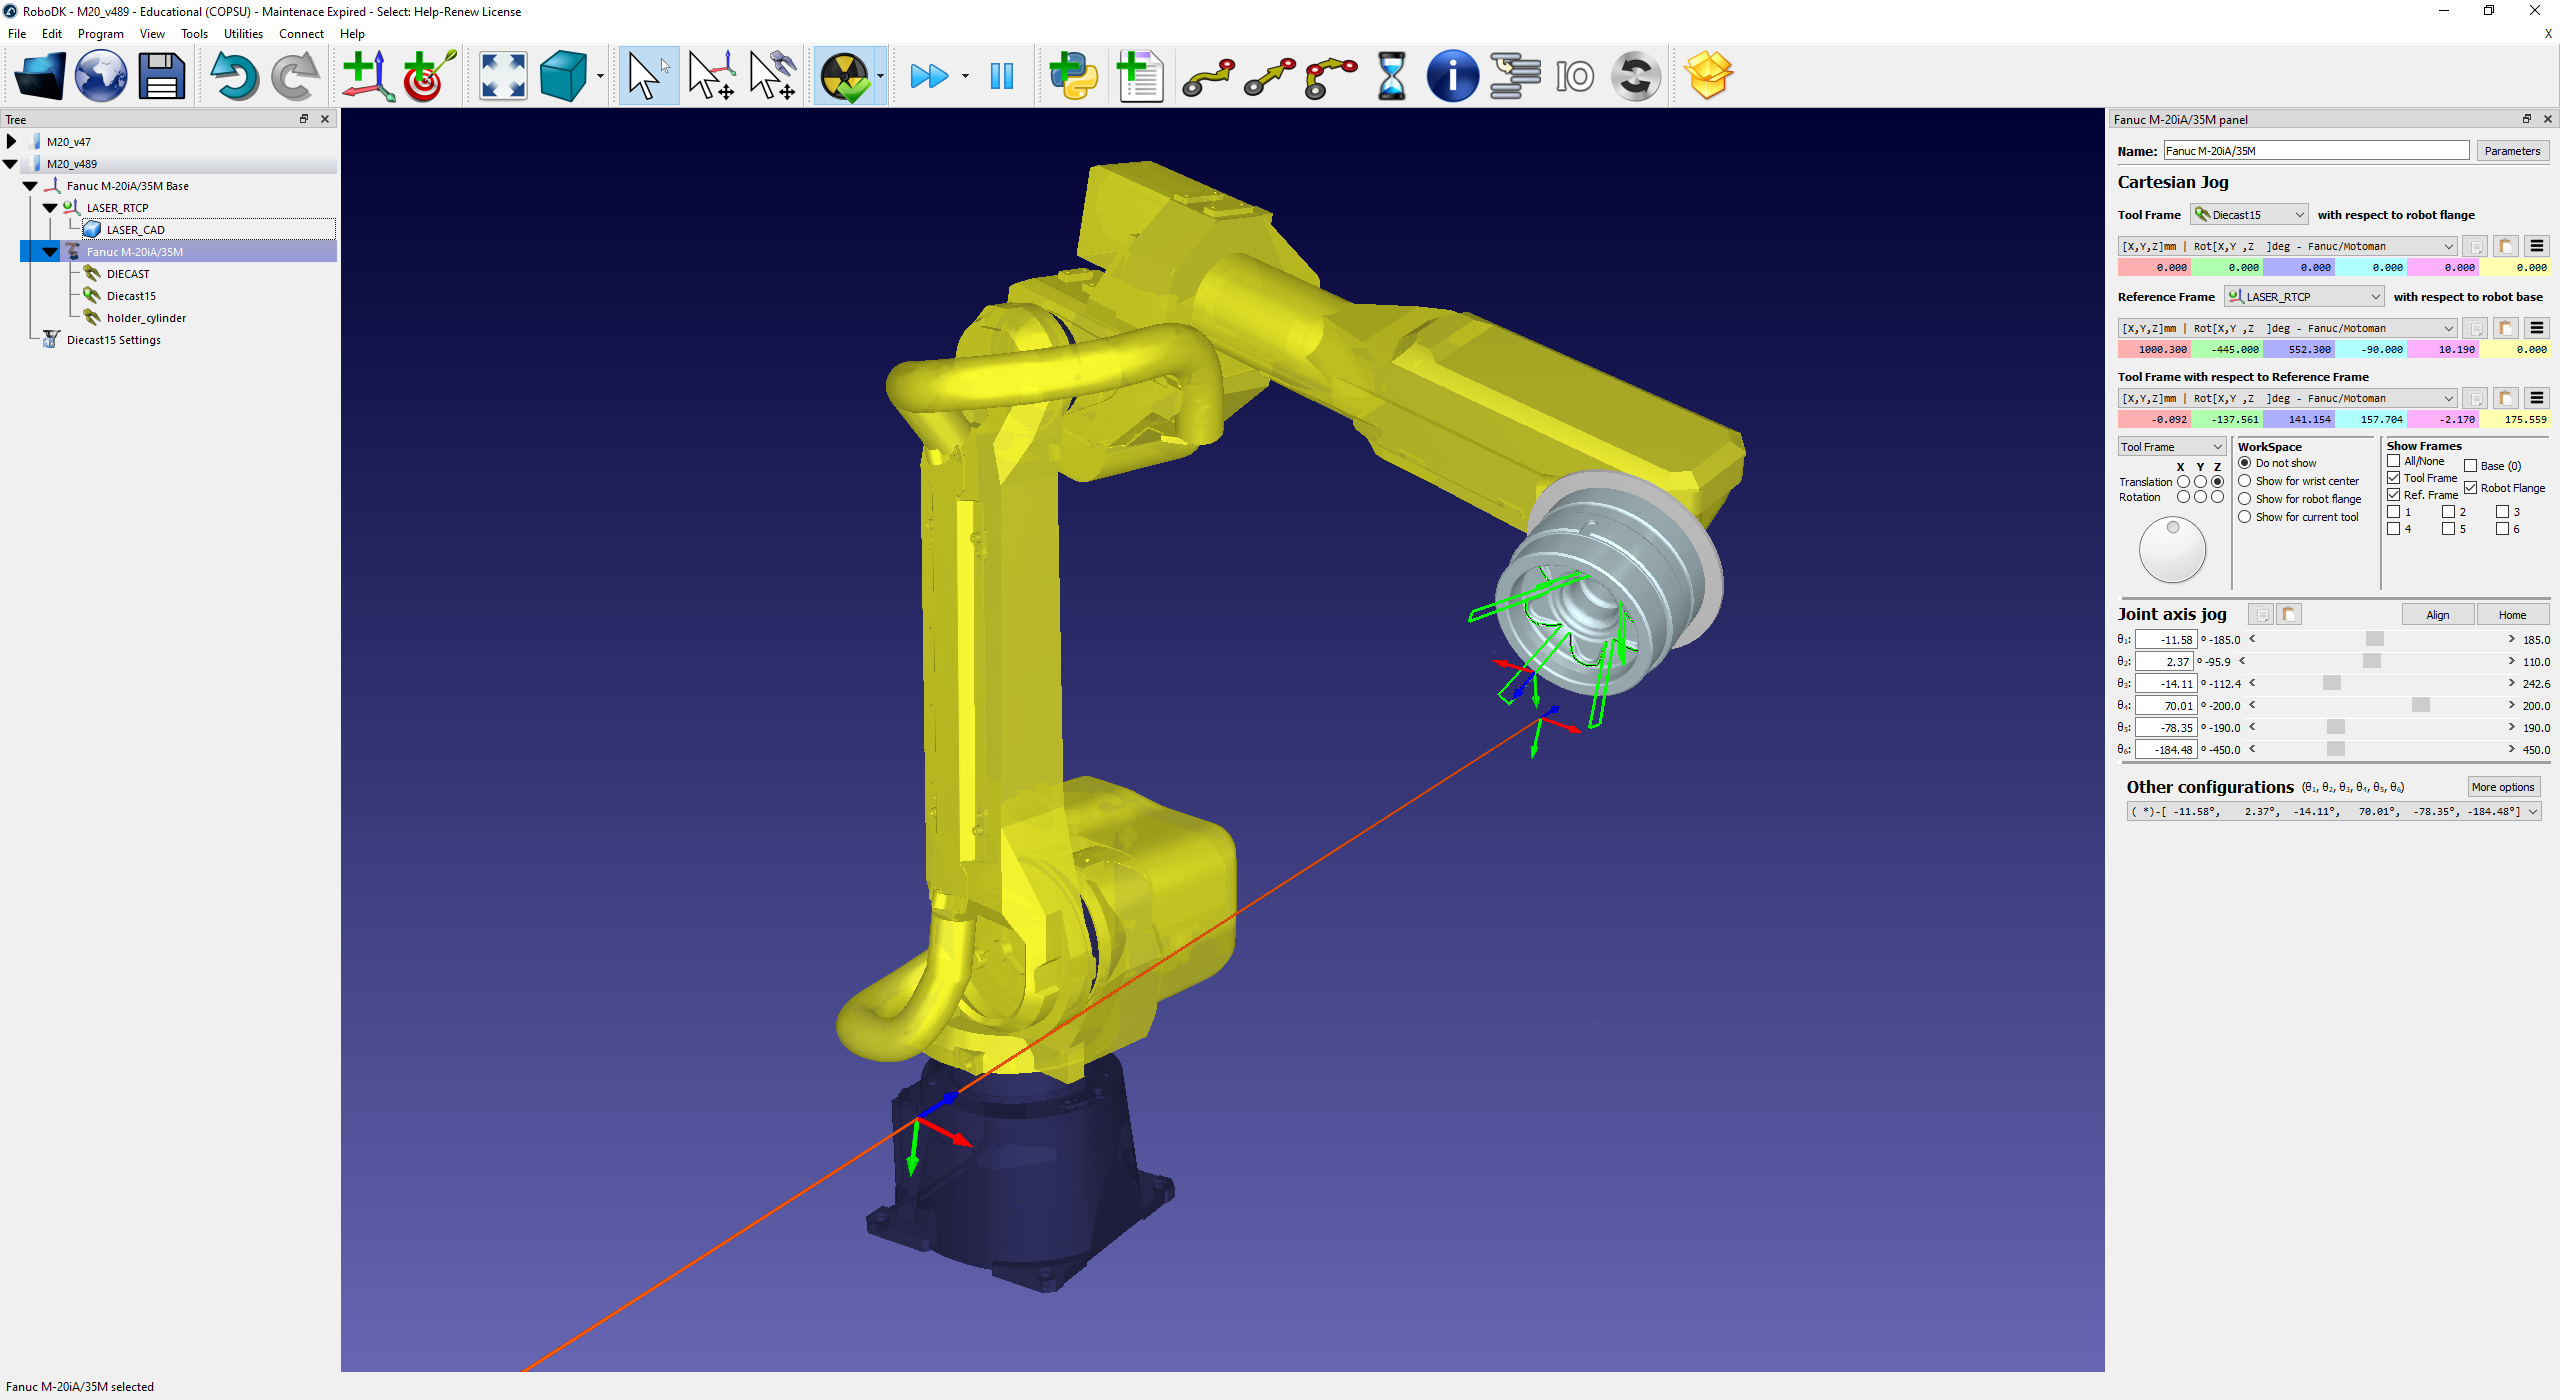
\includegraphics[width=0.8\linewidth]{img/robodk_cast.PNG}
    \caption{RoboDK workcell with forging die}
    \label{fig:robodk_die}
\end{figure}


\section{Testing on the physical robotic arm}

The testing of robotic arm programs on physical robotic arm succeeds the simulation process and is roughly divided into the following steps:

\begin{enumerate}
    
\item upload program to robotic arm controller,

\item run program on physical robotic arm in test mode (test mode = mode of robotic arm with reduced maximum speed) and without active laser source,

\item run program on physical robotic arm in production mode (production mode = speed of robotic arm is not restricted) and without active laser source,

\item run program in production mode with active laser source. The energy of the laser source is set to a~value that is appropriate for the given LSP application. 

\end{enumerate}
Figure~\ref{fig:cast} shows the forging die mounted on the robotic arm. The parameters chosen for the forging die experiment are listed in Table~\ref{experimental_forging}. 

\begin{table}[h!]
\centering
    \begin{threeparttable}
        \begin{tabular}{|c | c|} 
        \hline
            \textbf{Parameter} & \textbf{Value} \\ [0.5ex] 
        \hline
        Laser source & Litron LPY ST  \\
        \hline
        Wavelength [\SI{}{\nano\second}] & 1064 \\
        \hline
        Repetition Rate [\SI{}{\hertz}] & 1  \\ 
        \hline
            Pulse energy at sample [\SI{}{\milli\joule}] & 3200 \\
        \hline
            Beam size at sample [\SI{}{\mm\squared}] & 3.14 \\
        \hline
            Pulse Length @1064nm [\SI{}{\nano\second}] & 12 \\
        \hline
            Power density at sample [\SI{}{\giga\watt\per\cm\squared}] & 8.49 \\

        \hline
        \end{tabular}

        \caption{Experimental parameters of LSP process on \mbox{forging} die}
        \label{experimental_forging}
    \end{threeparttable}
\end{table}

\begin{figure}[h!]
    \centering
    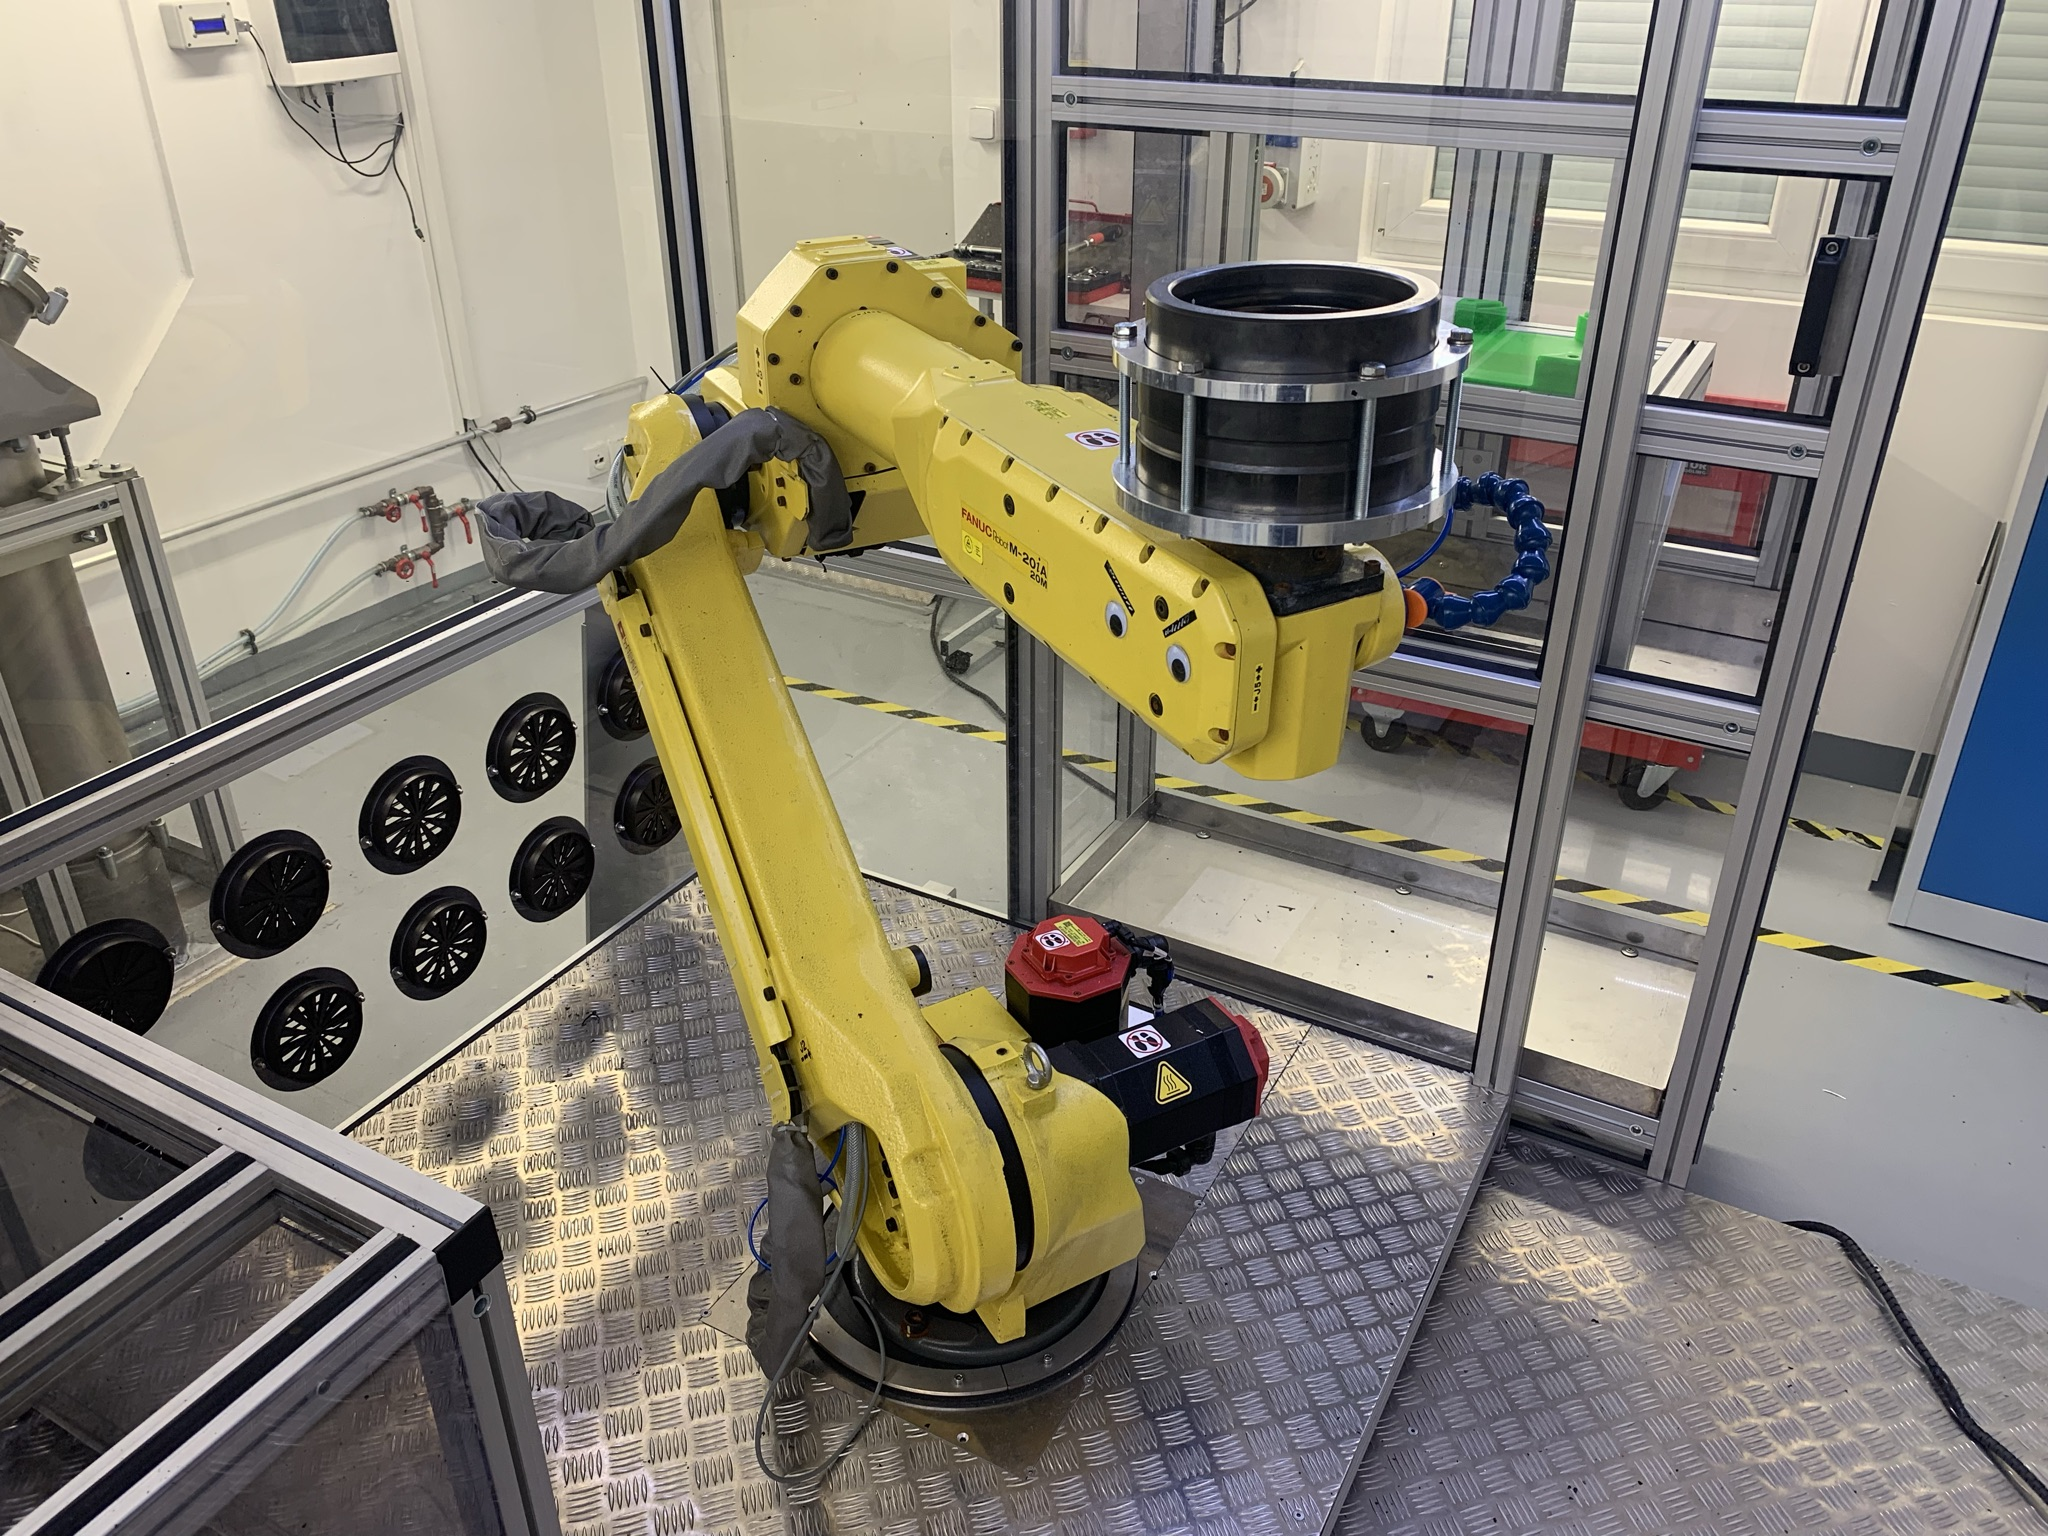
\includegraphics[width=0.9\linewidth]{img/cast.jpeg}
    \caption{Forging die mounted on the robotic arm}
    \label{fig:cast}
\end{figure}

\section{Results of simulation and testing}

\subsection{Results of simulation}

The simulation has been a~quick way of testing various ideas by changing the parameters of the simulation. The simulation has also allowed the author to create large programs with the number of points in the order of hundreds. Creating such large programs manually using a~teach pendant would be enormously time-consuming. 

Initially, the laser beam was parallel to the surface normal of the forging die. Then, the angle between the surface normal and the laser beam was changed to achieve a~collision-free simulation. The angle of impact is measured in relation to the surface normal of the forging die. As a~rule of thumb, an angle of impact of fewer than 15$^{\circ}$ does not affect the result of the LSP process.  A simulation that is sufficiently close to the actual LSP process was created, and the testing continued on the physical robotic arm.

\subsection{Results of testing on a~physical robotic arm}

Generally, the program from the simulation does not transition directly to the physical robotic arm due to minor differences between the simulated and physical workcell.  As a~consequence, some tweaks to the robotic arm program were necessary. Therefore, the following program parameters were alternated:

\begin{itemize}

\item the laser beam is tied to a~user frame -- this user frame origin was shifted,

\item the forging die was rotated around the J6 robotic arm joint (the J6 joint is responsible for the rotation of the robotic arm flange).
 
\end{itemize}
The testing on the physical robotic arm has been successful -- the LSP affected area on the surface of the forging die has matched the area to be treated by LSP specified in the simulation. Figure~\ref{fig:peening} shows the actual LSP process performed on the forging die. 

\begin{figure}[h]
    \centering
    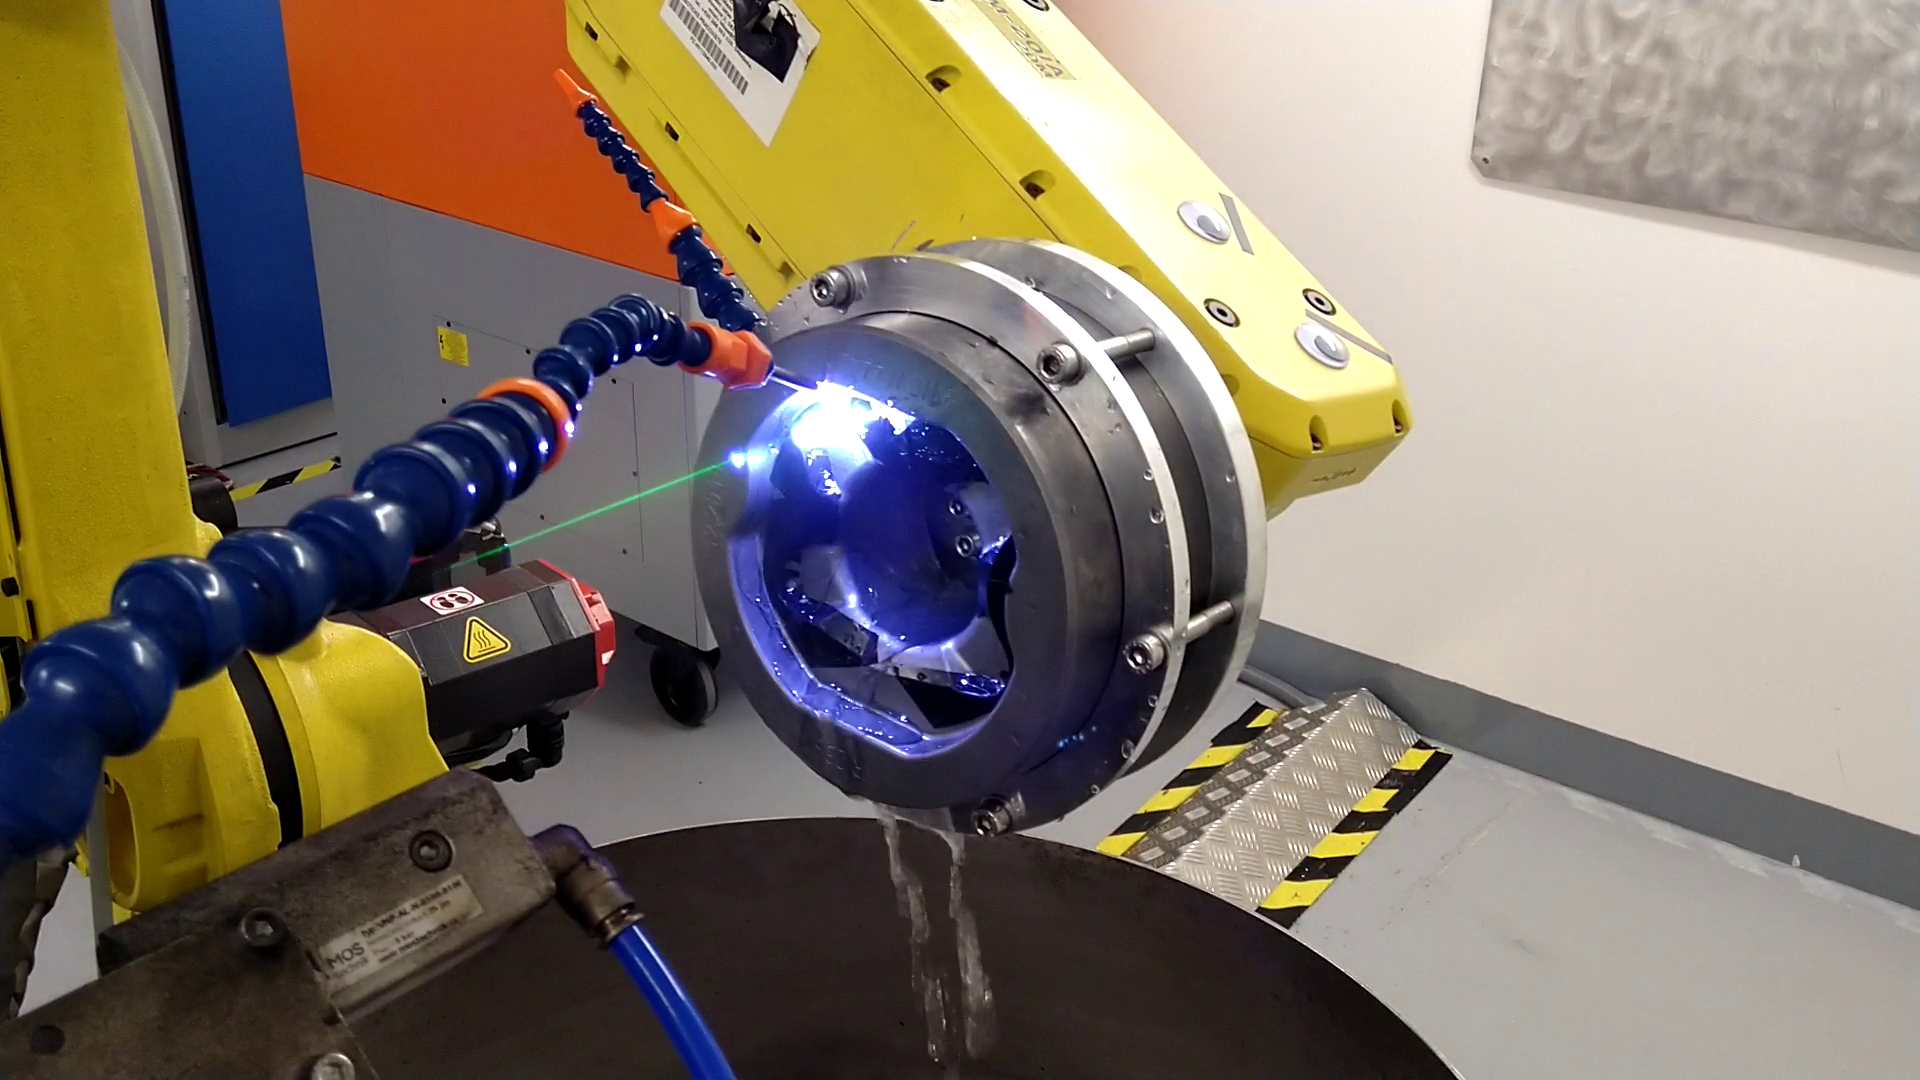
\includegraphics[width=0.9\linewidth]{img/peening_v2.png}
    \caption[LSP process performed on the forging die]{LSP process performed on the forging die with plasma emitting from the surface of the material}
    \label{fig:peening}
\end{figure}



